\section{Evaluation}
\label{sec:evaluation}
In this section, we present an experimental evaluation of \projecttitle.% based on the implementation described in  \secref{implementation}. 
%Our evaluation answers the following questions.
%
%\begin{itemize}
%\item What overheads does \projecttitle impose for recording data provenance? ($\S$~\ref{subsec:overheads})
%%\item How do these overheads scale with increases in the size of input data? ($\S$~\ref{subsec:data-sizes-overheads})
%\item What are the sources for the provenance overheads? ($\S$~\ref{subsec:overheads-breakdown})
%\end{itemize}

%Before answering these questions, we first describe the experimental setup used for the evaluation.

\begin{figure}[t]
\centering
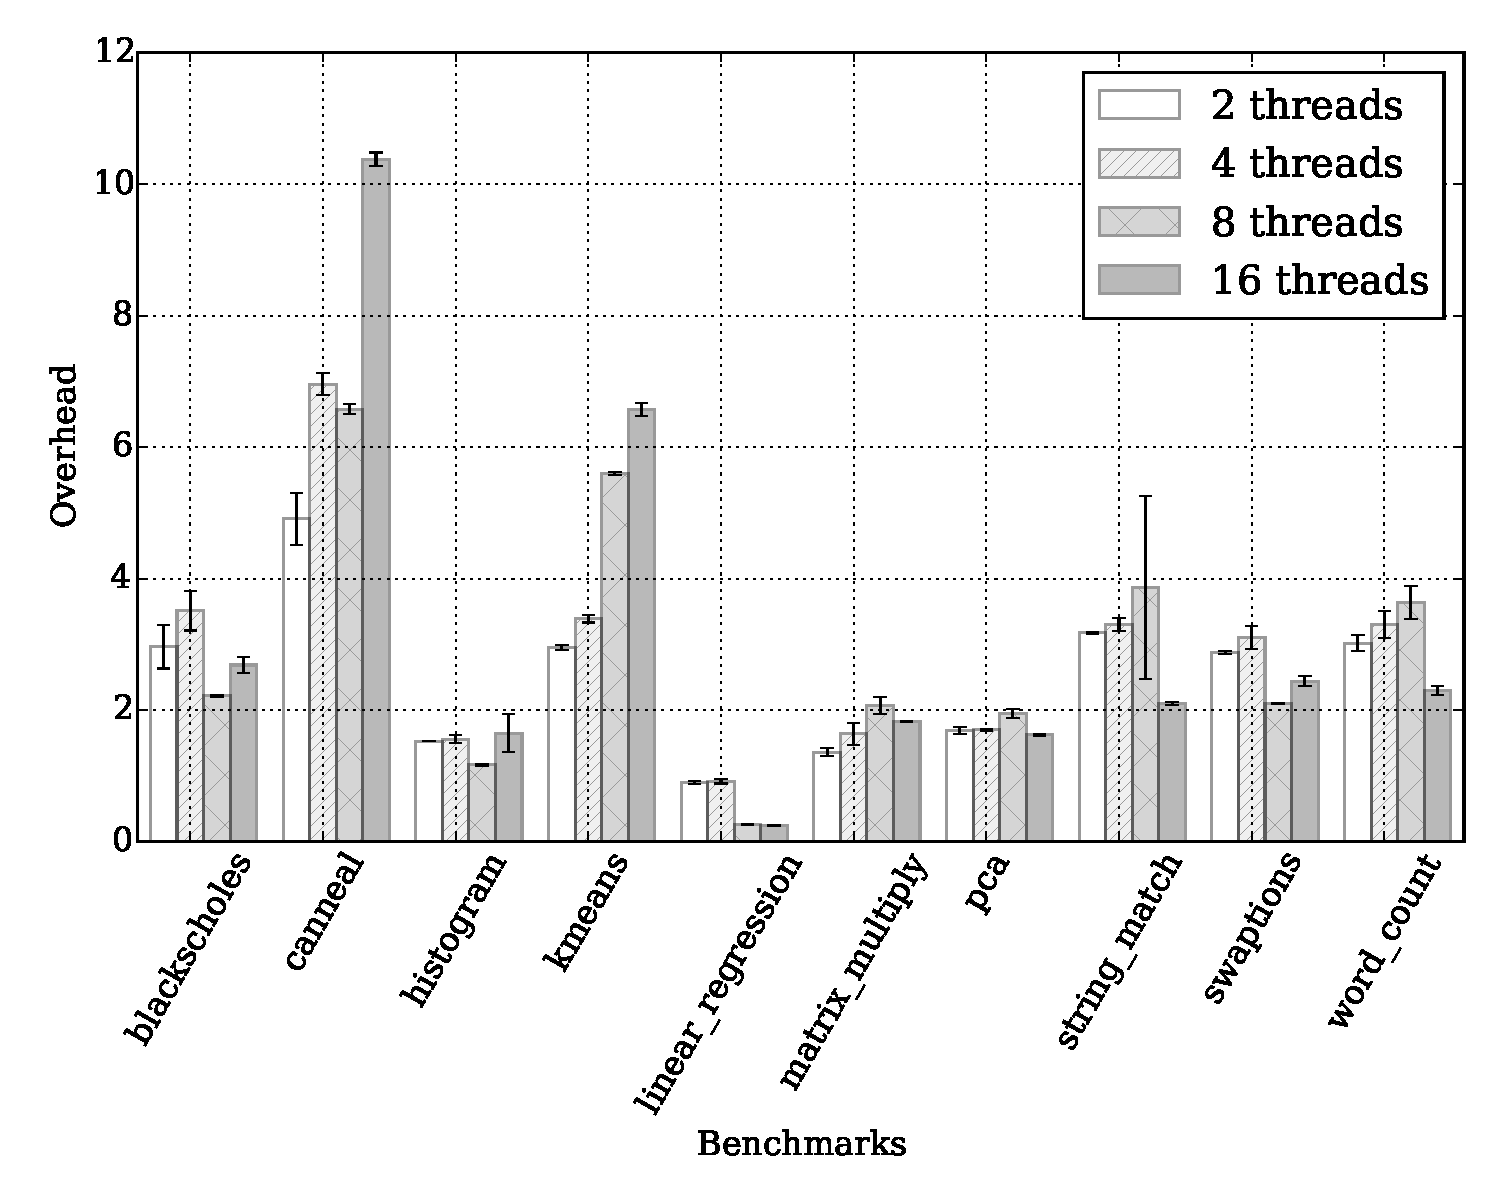
\includegraphics[scale=0.46]{figure/benchmarks/times-inspector.pdf}
\caption{Performance overhead  over native execution with increasing number of threads.}
\label{fig:overheads}
\end{figure}


%\subsection{Experimental Setup}


\myparagraph{Experimental platform} We used an Intel Xeon processor based
multicore architecture as our host machine for our evaluation. The
host system consists of 8 cores (16 hyperthreads) of Intel(R) Xeon(R) CPU Processor D-1540
(12M Cache, 2.00 GHz) and 32 GB of DRAM main memory. The host
machine is running Linux with kernel 4.3.0 in 64-bit mode. The log produced by
{\tt perf} was written to {\tt /tmp} on {\tt tmpfs} to allow high throughput.
%When varying the number of threads, we also regulate the numbers of active cpu cores.
%No additional core was provided for Perf.


\myparagraph{Applications and dataset}  We evaluated \projecttitle using two multithreaded benchmark suites: Phoenix 2.0 and PARSEC 3.0. 

%\myparagraph{Applications and dataset}  We evaluated \projecttitle using from two multithreaded benchmark suites: Phoenix 2.0 \cite{phoenix} and PARSEC 3.0 \cite{parsec}. %Table~\ref{tab:apps} lists the applications used for the evaluation along with the input data and benchmark parameters.
%

\myparagraph{Measurements}  For all experiments,  we report {\tt time}
measurements, i.e., run-time comparison, between the native {\tt pthreads}
execution, and \projecttitle execution.  All applications were compiled using
GCC 5.2.1 compiler with -$o3$ optimization flag. For all performance
measurements, we report the average over 6 runs with minimum and maximum values
discarded (truncated mean).

\myparagraph{Additional results} We also measured  {\em work} numbers, i.e., the overall CPUs utilization for all threads for both \pthreads and \projecttitle executions. (To measure work, we used the CPU accounting controller in {\tt cgroups} to account the CPU usage of all threads.) Due to space limitations, the work measurements are available online on the following anonymized link:  \href{https://goo.gl/0wp1kC}{https://goo.gl/0wp1kC}
%Due to the space limitation, we only present  time measurements for all experiments. 

%\myparagraph{Metrics: Time and Work}  We consider two types of measures to report the performance metrics: {\em time} and {\em work}. In a nutshell, time measurements reflect the end user perceived latency, whereas work measurements assess the overall resource (CPU) utilization.  More specifically,  time refers to the end-to-end computation time for the multithreaded applications. Work refers to the total computation performed by all threads, and it is measured as the cumulative CPU time for all threads. To measure work, we used the CPU accounting controller in {\tt cgroups} to account the CPU usage of all threads.

%\myparagraph{Measurements} All applications were compiled using GCC 5.2.1 compiler with -$o3$ optimization flag. For all performance measurements, we report the average over 10 runs with minimum and maximum values discarded.

%\myparagraph{Performance metrics: Work and Time}  For each run, we consider two types of measures: \emph{work} and
% {\em time}. Work refers to the total amount of
%computation performed by all threads and is measured as the total
%run-time of all threads. Time refers to the amount of (end-to-end)
%run-time to complete the parallel computation. Both metrics are important
%and complementary: time measurements reflect the end user perceived latency,
%whereas work measurements assess the overall resource (CPU) utilization.

\subsection{Provenance Overheads}
\label{subsec:overheads}
First, we explain the overheads imposed by \projecttitle for recording data provenance. In this respect, we present the provenance overheads w.r.t the native \pthreads execution with increase in the number of threads, and increase in the input sizes.


\myparagraph{Scalability with threads} Figure~\ref{fig:overheads} shows the provenance overheads of \projecttitle w.r.t. the native \pthreads execution with varying number of
threads (from $2$ to $16$ threads). As expected, the provenance overheads increases with the increase in the number of threads. This is because the shared memory commit ($\S$\ref{sec:impl-lib}) takes longer time with a higher number of threads. 

The experiment shows that the provenance overheads using \projecttitle vary across applications. 
We observe that a majority of applications ($9$/$12$) have a reasonable overhead between $1\times$ up to $2.5\times$ w.r.t. the native execution. However, three applications have exceptionally high overheads:  {\em canneal}, {\em reverse\_index}, and {\em kmeans}. The high overheads could be explained as follows: {\em canneal} modifies a lot of memory pages leading that leads to a high number of page faults for deriving read and write sets. Whereas, {\em reverse\_index} does a lot of small memory allocations across threads leading to a large number of segmentation faults.  Finally, {\em kmeans} creates more than $400$ threads in an iterative convergence algorithms. Since, processes take more time to create instead of threads, we see a slowdown in {\em kmeans}.


On the other hand, {\em linear\_regression} performs better than \pthreads, which is explained by the fact that our implementation of threads as processes ($\S$\ref{sec:implementation})  avoids false sharing, as previously noted by Dthreads~\cite{dthreads-sosp-2011}.



Lastly, in the case of {\em streamcluster}, we were limited by our physical memory to store the log in {\tt tmpfs} for $16$ threads. Therefore, we also show the overheads with $14$ and $15$ threads,  where the provenance log can fit into the main memory.  %To better understand the breakdown of provenance, we chose $15$ threads for {\em streamcluster} in $\S$~\ref{subsec:overheads-breakdown}.


%The overhead of collecting processor trace while using native
%\pthreads was 2 slower on average and there for causes an
%significant part of the of the slowdown.

%In {\tt Canneal} and {\tt Reverse Index} a high number of pages were modified.
%Reverse index does a lot of small memory allocations across the threads. This
%leads to more segmentation faults, because these allocations are located on
%different pages. In Kmeans during execution over 1000 threads were created. As
%processes take more time to create instead of threads, we see a slowdown here as
%well.
%
%For linear regression a speedup was measured. Because in this execution model,
%every “thread” has its own virtual memory: No cohearence protocol has to be run
%between commits. This prevents false sharing which results in a speedup even
%when recording the execution trace.

%The provenance overheads increases with the increase in the number of threads.
%This was expected, because the serial phase between memory commits takes longer,
%with a higher number of threads. 

%
%In Streamcluster, we were hitting the memory
%limit to store the log in {\tt tmpfs} for 16 threads. To better understand the
%breakdown we chose 15 threads in Figure~\ref{fig:overheads}, where the log can
%fit into the main memory. 


%\label{subsec:data-sizes-overheads}

\begin{figure}[t]
\centering
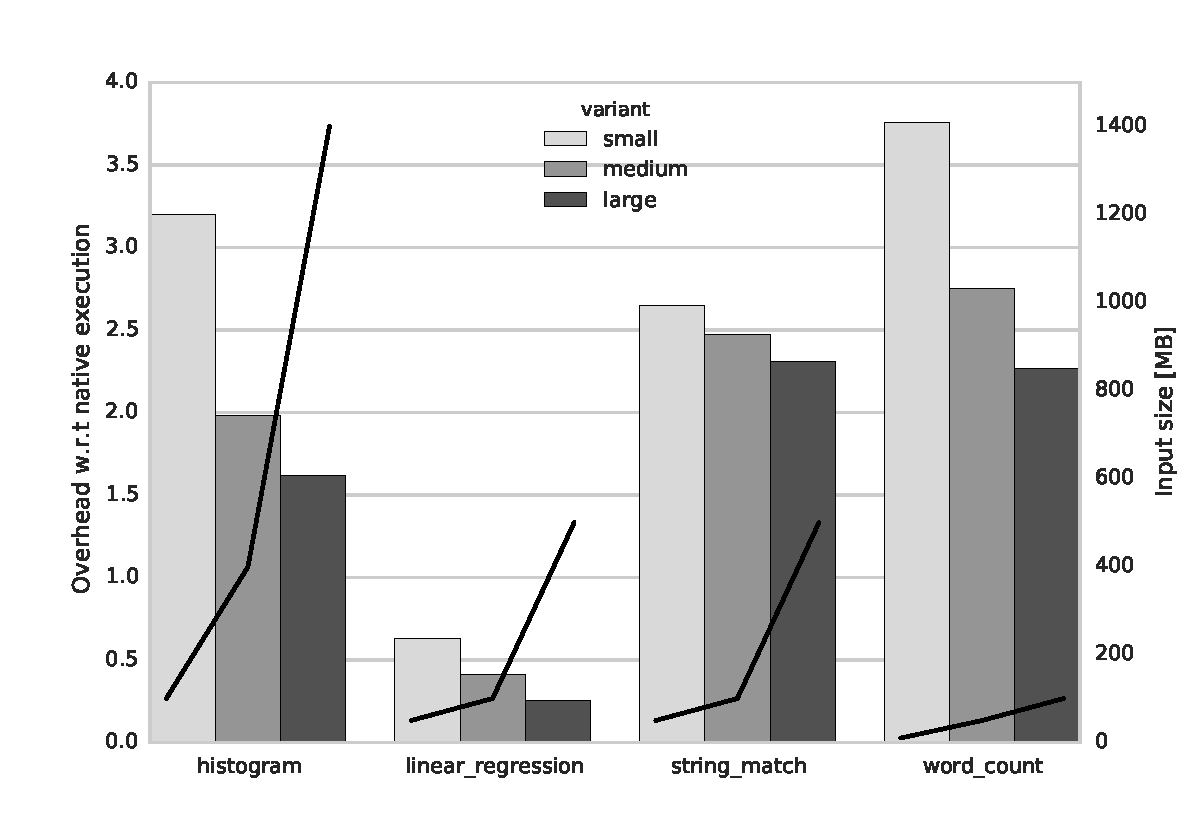
\includegraphics[scale=0.3]{figure/benchmarks/worksize-times-xy.pdf}
\caption{Scalability of overheads with increase in the input data sizes with $16$ threads. }
\label{fig:data-size-overheads}
\end{figure}

\myparagraph{Scalability w.r.t. input data sizes} In addition to scalability w.r.t.  threads, we also measured the performance overheads with increases in the size of the input.  For that, we
report the performance overheads for four applications ({\em histogram}, {\em linear\_regression}, {\em string\_match}, and {\em word\_count}) that are available with
three input sizes: small ($S$), medium ($M$), and large ($L$).


Figure~\ref{fig:data-size-overheads} shows a bar plot of the performance overheads w.r.t. to the native \pthreads execution. For the reference, the input sizes are also shown by a line plot in the same figure on the $Y2$ axis. The result shows that the gap between \pthreads and \projecttitle narrows with bigger input sizes. This is due to the fact that most applications use a data-parallel programming model for parallelization, where the main threads divides the input data evenly between the worker threads. As the input size increases, each thread spends relatively more time outside the shared-memory commit to compute on the data, and therefore, it results in improved performance.
 

%
% algorithms used here divide input evenly between the
%threads. As the input size increase therefor the parallel phase increases and
%the overhead of the memory commit gets smaller in relatively.





\subsection{Overheads Breakdown}
\label{subsec:overheads-breakdown}
Next, we present  the sources for the provenance overheads. \projecttitle imposes two types of overheads: (1) performance overheads, and (2) space overheads for storing the provenance graph.


\myparagraph{Performance overheads} Figure~\ref{fig:overheads-breakdown} shows the breakdown of overheads with $16$ threads normalized to the native \pthreads execution. We quantify the breakdown as the time taken by the \projecttitle library ($\S$~\ref{sec:impl-lib}) and the OS support for \intelpt  ($\S$~\ref{sec:impl-OS}). The result shows an interesting pattern: the applications with unreasonably high overheads ({\em canneal}, {\em reverse\_index}, and {\em kmeans}) spend a majority of time in the \projecttitle library. Whereas, the processor trace overheads is a dominant factor for the other applications with the reasonable provenance overheads.



\begin{figure}[t]
\centering
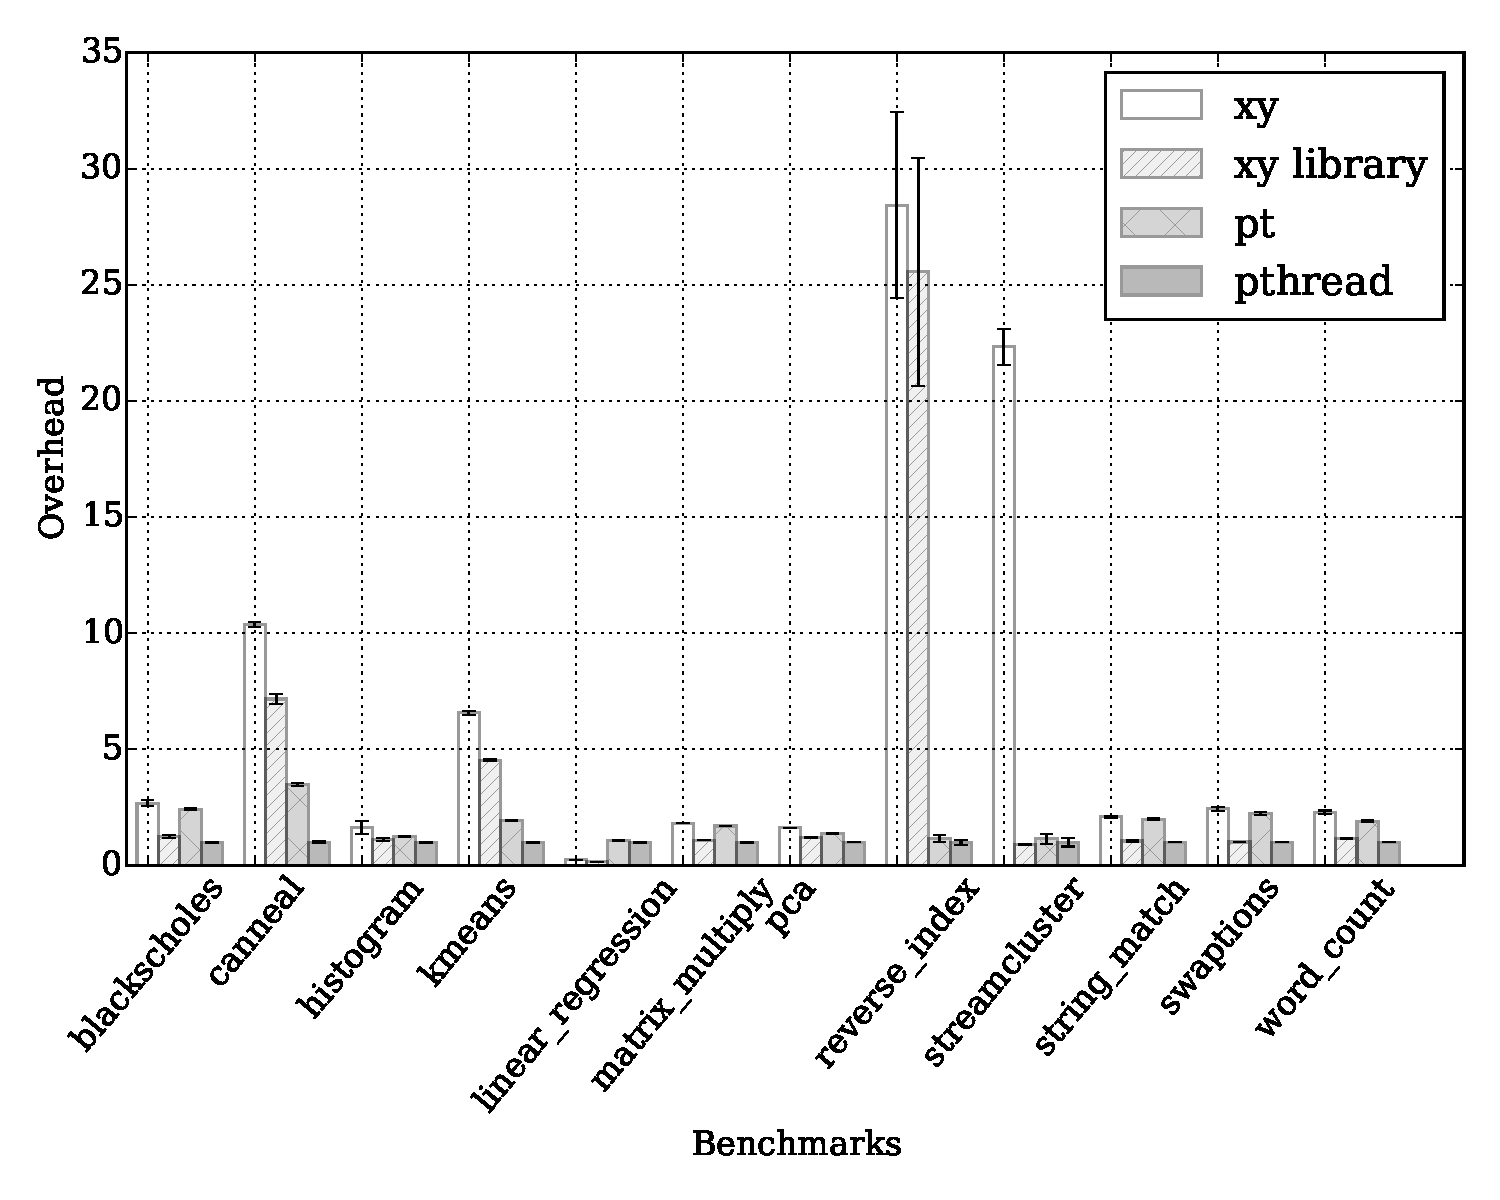
\includegraphics[scale=0.43]{figure/benchmarks/times-16-threads.pdf}
\caption{Performance overhead breakdown with $16$ threads --- except for streamcluster, where overhead for 15 threads is shown}
\label{fig:overheads-breakdown}
\end{figure}



\myparagraph{Space overheads} We also measured the space overheads for the provenance trace. Table~\ref{tab:apps} shows the space overheads for all applications with~$16$ threads. The provenance log written by {\tt perf} turns out to be highly compressible. We
are able to achieve a compression ratio of between $6\times$ and $37\times$ times using the lz4 compression algorithm.
\begin{figure}[t]
\centering
\myfontsize
\newcommand{\tworowcell}[2][c]{\begin{tabular}[#1]{@{}c@{}}#2\end{tabular}}
{
%\begin{tabular}{l | r r r r}
%[-8pt]
 % {\bf Application} & {\bf Compressed log size [MB]} & {\bf Log bandwith [MB/s]}& Branch instr. \\
\begin{tabular}{m{1cm}|m{1cm}|m{1.4cm}|m{1.25cm}|m{1.25cm}}
 &   \multicolumn{2}{c|}{ Provenance log details [MB] }   & \multicolumn{2}{c}{ Breakdown [MB] } \\
   { Application} & Size & Compressed & Thread lib. &  OS support \\
  \hline \hline
    blackscho. 	&	851		& 57.3 (14.9$\times$)	&  2.404E+09& 1644  \\
    canneal  	&	5343		& 315  (17.0$\times$)	&  1.512E+10& 947672   \\
    histogram 	&	381 		&  11.3	( 33.6$\times$)	&  1.651E+09& 102   \\
    kmeans 	&	1.19E+04 	& 522	(22.8$\times$)	&  4.803E+10& 481947   \\
    linear\_reg 	&	183 		& 5.46	(33.5	$\times$)&  9.881E+08& 52   \\
    matrix\_mul 	&	2101  	& 97.0	(21.7$\times$)	&  8.067E+09& 3977   \\
    pca		& 	1900 	& 116	(16.4$\times$)	&  7.408E+09& 241404   \\
    reverse\_idx	&	192 		& 5.70	(33.7	$\times$)&  4.564E+08& 262  \\
    streamcl.	&	2.93E+04 & 787	(37.3$\times$)	&  1.095E+11& 15703  \\
    string\_ma.	&	2751		& 430	(6.4$\times$)		&  8.749E+09& 53  \\
    swaptions	&	7061		& 929	(7.6$\times$)		&  1.867E+10& 1018  \\
    word\_c.	&	4121		& 508	(8.1$\times$)		&  8.047E+09& 21709  \\
\hline
\end{tabular}
}

\caption{Runtime statistics of benchmarks with 16 threads (Detailed results available here: \href{https://goo.gl/UgPNdS}{goo.gl/UgPNdS}) }
\label{tab:apps}
\end{figure}

